\documentclass[hyperref={bookmarksopen=false}]{beamer} 

\usepackage[english]{babel}
\usepackage{pgf,pgfarrows,pgfnodes,pgfautomata,pgfheaps,pgfshade}
\usepackage{ngerman}
\usepackage[latin1]{inputenc}

\usepackage{graphicx}

\useoutertheme[section]{tubs}

%\setbeamertemplate{itemize items}[ball]
%\setbeamertemplate{itemize items}[square]
\setbeamertemplate{itemize items}[tusquare]

\subtitle{Labor Android Programmierung - 2. Review}
\title{LDAP Contact Sync} 
\author[C. Gerloff und T. Lorentzen]{Till Lorentzen und Christopher Gerloff}
\institute[TU Braunschweig, IBR]{Technische Universit�t Braunschweig, IBR}

\date{\today}

\instlogo{ibr_deu}
%\titlegraphic{iz}
\titlegraphic{iz_corner}



\begin{document}

\frame[plain]{\titlepage} 

\setbeamercolor{frametitle}{fg=white,bg=tu-red}
\frame{
        \frametitle{Einleitung}
        \tableofcontents
        }
\setbeamercolor{frametitle}{fg=black,bg=tu-grey}


\section{Projektziel}

\frame{
 \frametitle{Synchronisation mit LDAP Kontakten} 
 \begin{block}{Anforderungen}
 \begin{itemize}
    \item Verbindung zu Server herstellen
    \item Kontakte des LDAP Servers durchsuchen
    \item Kontakte importieren
    \item Importierte Kontakte mit vorhandenen Kontakten zusammenf�hren
    \item �nderungen synchronisieren

 \end{itemize}
 \end{block}
}

\section{Stand der Dinge}
\frame{
	\frametitle{Stand der Dinge}
	
 	  \begin{block}{Bisherige Ergebnisse}
   	      \begin{itemize}
                  \item LDAP Bibliothek: 
                    \begin{itemize}
                      \item LDAP SDK von UnboundID
                    \end{itemize}
                  \item Importieren funktioniert
		  \item neue Kontakte im LDAP werden automatisch im Kontaktbuch erstellt
		  \item Kontakte l�schen ist implementiert
		  \item Exportieren/Synchronisieren in Arbeit
                  \item Grafischen Oberfl�che erstellt
                  \item LDAP Server l�uft
                \end{itemize}
           \end{block}
}

\section{�nderungen}
\frame{
 \frametitle{Wichtige Komponenten} 
\begin{block}{RawContacts}
    \begin{itemize}
        \item Kontaktdaten werden pro Account gespeichert
	\item Sichtbarkeit im Kontaktbuch je nach Wunsch 
    \end{itemize}
 \end{block}
 \begin{block}{SyncAdapter}
    \begin{itemize}
        \item Schnittstelle f�r Android zur Synchronisation
    \end{itemize}
 \end{block}

   \begin{block}{ContentProvider}
    \begin{itemize}
        \item Ersetzt durch LDAPSyncService
    \end{itemize}
 \end{block}
}

\frame{
\frametitle{Contact Database}
  \begin{block}{Datenstruktur der Kontakte}
    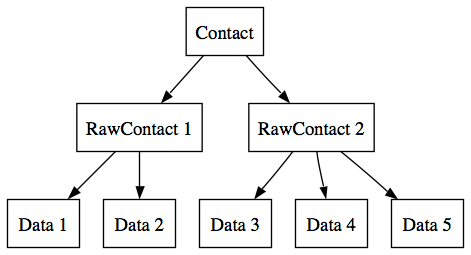
\includegraphics[width=0.8\textwidth]{contacts-2.png}\\
    \tiny{Quelle: http://developer.android.com/resources/articles/contacts.html}
  \end{block}

  
}
\frame{
\frametitle{RawContacts}
  \begin{block}{Synchronisationsfelder in den Kontakten}
    \begin{itemize}
      \item ACCOUNT NAME = Account.name
      \item ACCOUNT TYPE = Account.type
      \item SOURCE ID = entryUUID
      \item SYNC1 = Sync Status
      \item SYNC2 = DN \& LDAPObjectClasses
      \item SYNC3 = LDAP Fehlermeldungen
      \item SYNC4 = LDIF der letzten erfolgreichen Synchronisation
    \end{itemize}
  \end{block}  
}

\frame{
\frametitle{Sync Status}
  \begin{block}{M�gliche Zust�nde}
    \begin{itemize}
      \item locally added
      \item locally changed (implizit: DIRTY is true)
      \item locally deleted (implizit: DELETED is true)
      \item remote added (muss nicht bedacht werden: funktioniert automatisch)
      \item remote changed (implizit: diff (LDAP Entry, LDIF in SYNC4) )
      \item remote deleted (implizit: SOURCEID ist nicht auf dem LDAP \& Status != locally added)
      \item in sync
      \item change conflict
    \end{itemize}
  \end{block}  
}

\frame{
	\frametitle{Grafische Oberfl�che}
	\begin{block}{Hauptbildschirm}
	\hspace{0.5 cm}
 	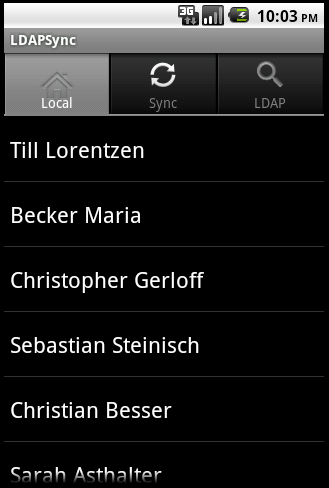
\includegraphics[scale=0.3]{TabView.png}
	\vspace{1 cm}
 	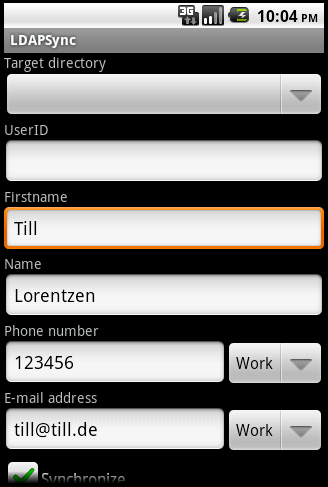
\includegraphics[scale=0.3]{DetailView.png}
	\vspace{1 cm}
 	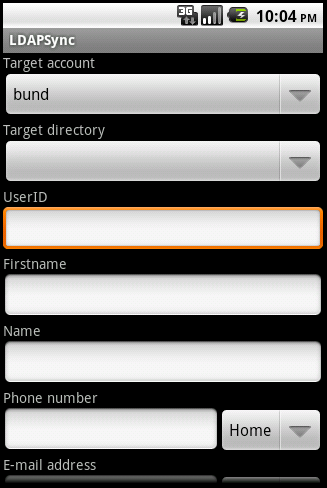
\includegraphics[scale=0.3]{AddContact.png}
	\end{block}
}

\frame{
  \frametitle{Teamwork}
  \begin{block}{Git \& GitHub}
    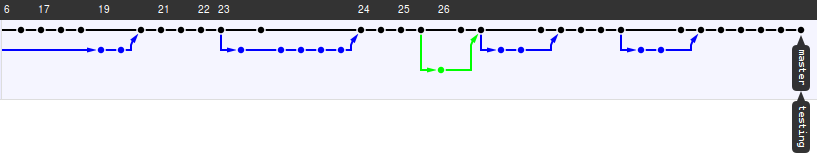
\includegraphics[scale=0.35]{git.png}\\
    \tiny{ https://www.github.com/soneyworld/AndroidLab}\\
    \tiny{\$ git clone git://github.com/soneyworld/AndroidLab.git AndroidLab}
  \end{block}
  \begin{block}{Projektstatus}
    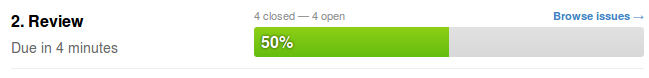
\includegraphics[scale=0.4]{status.png}\\
    \tiny{ https://github.com/soneyworld/AndroidLab/issues/milestones}
  \end{block}
}



\section{Ausblick}

\frame{
 \frametitle{Ausblick} 
 \begin{block}{To Do}
 \begin{itemize}
    \item Merge und Sync Prozesse
    \item Testen
    \item SyncTab implementieren
    \item Kontakteditor vervollst�ndigen
 \end{itemize}
 \end{block}
}

\frame{
  \frametitle{Fragen?}
  \begin{block}{Antworten!}
   
  \end{block}

  \begin{block}{Weitere Informationsquellen}
  \begin{itemize}
    \item Wiki: \tiny{https://github.com/soneyworld/AndroidLab/wiki}\normalsize
    \item Twitter: \tiny{https://twitter.com/ldapsync}
  \end{itemize}
  \end{block}
}

\end{document}   
